\section{545 --- Boundary of Binary Tree}
Given a binary tree, return the values of its boundary in \textbf{anti-clockwise} direction starting from root. Boundary includes left boundary, leaves, and right boundary in order \textbf{without duplicate nodes}.  (The values of the nodes may still be duplicates.)

\textbf{Left boundary} is defined as the path from root to the \textbf{left-most} node. \textbf{Right boundary} is defined as the path from root to the \textbf{right-most} node. If the root doesn't have left subtree or right subtree, then the root itself is left boundary or right boundary. Note this definition only applies to the input binary tree, and not applies to any subtrees.

The \textbf{left-most} node is defined as a \textbf{leaf} node you could reach when you always firstly travel to the left subtree if exists. If not, travel to the right subtree. Repeat until you reach a leaf node.

The \textbf{right-most} node is also defined by the same way with left and right exchanged.

\paragraph{Example 1}

\begin{flushleft}
\textbf{Input}:
\begin{figure}[H]
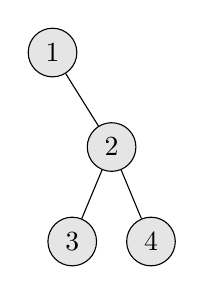
\begin{tikzpicture}
[every node/.style={draw, circle, fill=gray!20!, minimum size=5mm},
level 2/.style ={sibling distance=1cm}, 
level 3/.style={sibling distance=8mm},
level distance=1.2cm]
\node{1}
child[missing]
child{node{2} child{node {3}} child{node{4}}};
\end{tikzpicture}
\end{figure}

\textbf{Output}: $[1, 3, 4, 2]$

\textbf{Explanation}:

The root doesn't have left subtree, so the root itself is left boundary.

The leaves are node 3 and 4.

The right boundary are node 1, 2, 4. Note the anti-clockwise direction means you should output reversed right boundary.

So order them in anti-clockwise without duplicates and we have $[1,3,4,2]$.
\end{flushleft}


\paragraph{Example 2}

\begin{flushleft}
\textbf{Input}:
\begin{figure}[H]
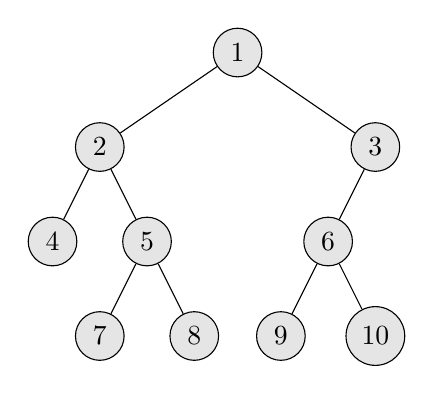
\begin{tikzpicture}
[every node/.style={draw, circle, fill=gray!20!, minimum size=5mm},
level 1/.style ={sibling distance=3.5cm}, 
level 2/.style={sibling distance=2.0cm},
level 2/.style={sibling distance=1.2cm},
level distance=1.2cm]
\node{1}
child{node{2} child{node{4}} child{node{5} child {node{7}} child {node{8}}}}
child{node{3} child{node{6} child{node{9}} child{node{10}}} child[missing]};
\end{tikzpicture}
\end{figure}
      
\textbf{Output}: $[1,2,4,7,8,9,10,6,3]$

\textbf{Explanation}:

The left boundary are node 1, 2, 4. (4 is the left-most node according to definition)

The leaves are node 4, 7, 8, 9, 10.

The right boundary are node 1, 3, 6, 10. (10 is the right-most node).

So order them in anti-clockwise without duplicate nodes we have $[1,2,4,7,8,9,10,6,3]$.
\end{flushleft}
